
In this section I provide the main results of the paper by replicating the a subset of Tables and Figures of the paper. All the codes can be found in the main folder in which this file is contained.

\subsection{One-Year Return Forecasts Mixing FB and GSW data}

\begin{table}[h!]
	\centering
	\caption{$R^2$ values for forecasting average (across maturity) excess returns $\bar{rx}_{t+1} = \frac{1}{14}\sum_{n=2}^{15}$. GSW denotes Gürkaynak, Sack, and Wright (2006) forward rate data. FB denotes Fama Bliss (1986) data, updated by CRSP. f1-f5 uses one to five year forward rates; f1, f3, f5 use only the one, three, and five year forward rates; f1-f15 use only the one, three, and five year forward rates; f1-f15 uses one to 15 year forward rates. 3 mo. MA uses three month moving averages of the right hand variables. Overlapping monthly observations of one-year return forecasts 1971-2006.}\label{tab:1}
	\input{tab/table1.txt}
\end{table}


For instance, Table \ref{tab:1} presetns the $R^2$ values of forecasting \textbf{one-year} returns in the GSW data from forward rates. The goal of these regression is trying to reduce the number of right hand variables to avoid multicollinearity. The main regressions here follow thus the form
\begin{equation}
	\bar{rx}_{t+1} = \alpha + \sum_{k=1}^{\#\mathcal{F}}\beta_k f_{t}^{(k)} + \varepsilon_{t+1},
\end{equation}
where $\mathcal{F}$ denotes here a certain set of forward rates. My results are pretty similar to those in the paper. Probably the highest difference is in the first row fourth column, in which I get an $R^2$ of 0.184 and they get $0.31$. The second highest difference is in the last row second column, in which I get 0.322 and they get 0.29. In general, my results don't differ more than 0.01 to those in the paper. In any case, I get the same pattern conssiting in an increase in the $R^2$ when using $f^{FB}$ instead of $f^{GSW}$ in the right hand side, which indicates that there are ill effects of smoothing across maturities in the GSW data. Hence, according to these results, I arrive to the same conclusion than Cochrane and Piazzesi: the 5 Fama-Bliss forward rates capture all the information in the 15 GSW forward rates about future returns, and more.

\subsection{The Return-Forecasting Factor $x$}

\begin{figure}[h!]
	\centering
	\caption{Factors in the covariance matrix of expected returns, regressing the 15 GSW returns on the 5 FB forward spreads.}\label{fig:3}
	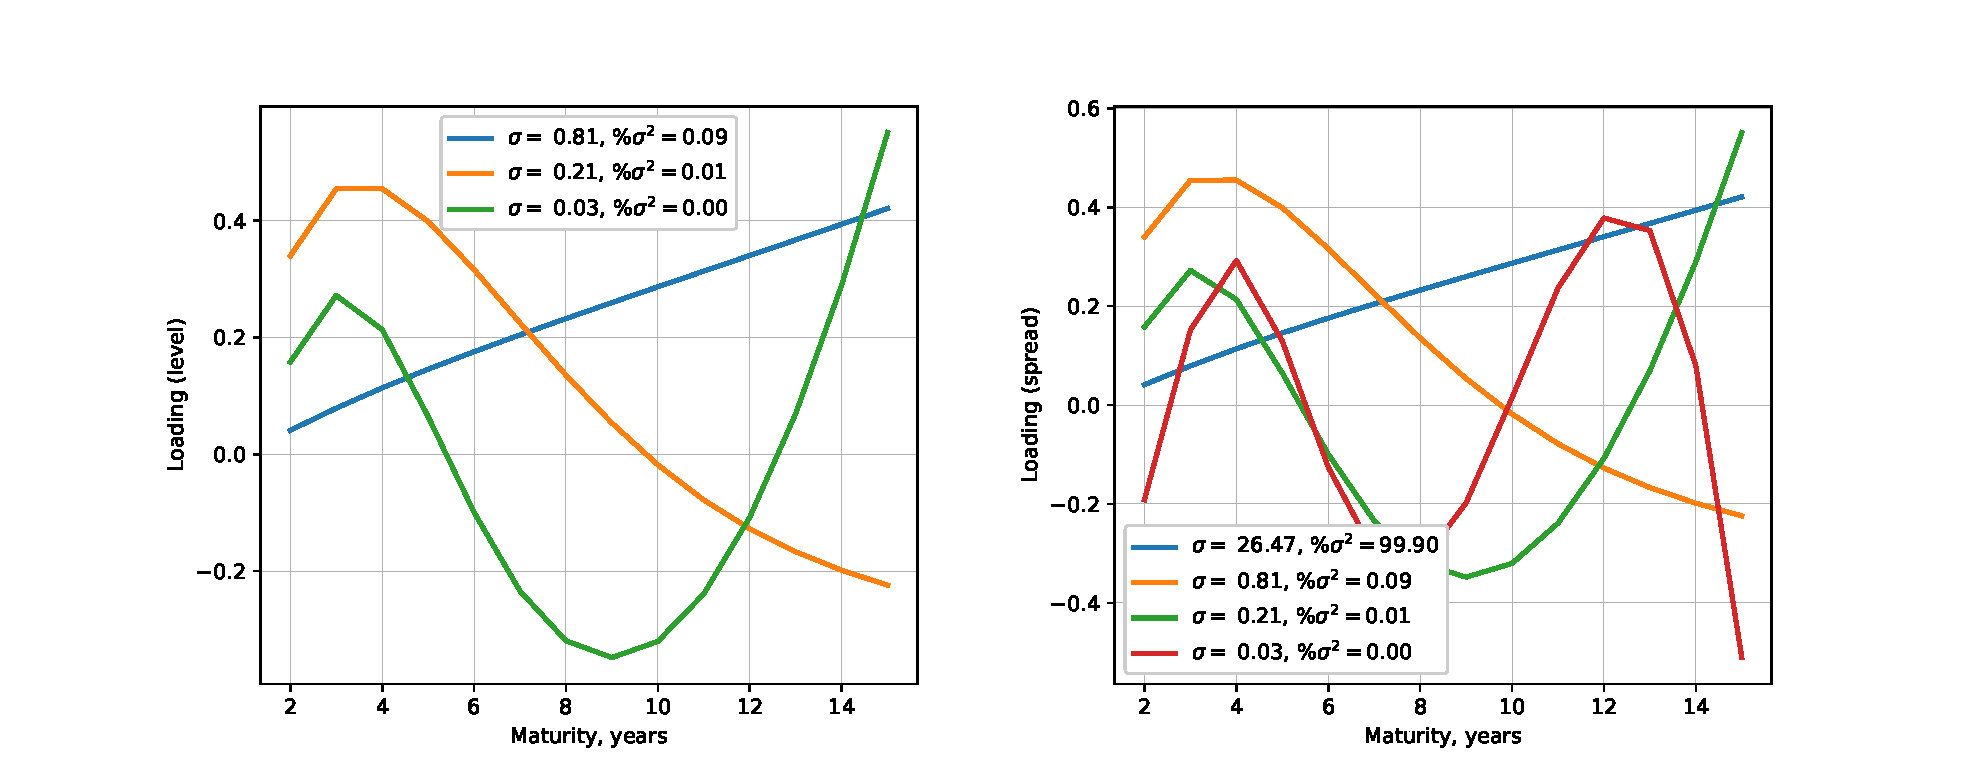
\includegraphics[scale=0.5]{fig/eps/Figure3.eps}
\end{figure}


Now what I will do is to construct the return-forecastnig factor in the same way that they do. To do so, I allow in my code for using either spreads or levels in the forward rates, i.e., either
\begin{equation}
	rx_{t+1}^{GSW} = \alpha + \beta f_t^{FB} + \varepsilon_{t+1}
\end{equation}
or
\begin{equation}
	rx_{t+1}^{GSW} = \alpha + \beta \tilde{f}_t^{FB} + \varepsilon_{t+1},
\end{equation}
where $f_t^{(n)} = f_t^{(n)} - y_t^{(1)}$. Note that $\tilde{f}_t$ starts when maturity is two years, since $\tilde{f}^{(1)} = 0$. The excess returns are taken as a three month moving average (4th row last row in Table \ref{tab:1} specification). In any of these specifications, we decompose the covariance matrix of expected returns in its eigenvalue matrix, i.e.,
\begin{equation}
	\text{cov}\left(\beta\tilde{f}_t^{FB}\right) = Q_r \Lambda_r Q_r^\T,
\end{equation}
where $\beta\tilde{f}_t^{FB}\ = \E_t\left[rx_{t+1}^{GSW}\right]$. The loadings (columns of $Q_r$) are plotted in Figure \ref{fig:3}. These loadings express how much expected excess reutrns of each maturity move when the corresponding factor moves. They are basically regression coefficients of expected returns on the factors. The caption gives the standard deviations of the factors $\sigma_i = \sqrt{\Lambda_{ri}}$ (where $\Lambda_{ri}$ is the $i$th eigenvalue\footnote{The eigenvalues in the matrix $\Lambda$ are ordered from highest to lowest.}) and the fractions of variance $\sigma_i^2 = \Lambda_{ri} / \sum_{j} \Lambda_{rj}$. I find as they do that the first factor utterly dominates this covariance matrix of expected returns, accounting for 99.9\% of the variance of exepcted returns. This basically means that almost nothing is changed by imposing a single-factor model. Note that the shape of some loadings across maturities is the opposite that the corresponding one in the paper. This is due to the fact that the eigenvector decomposition is the same modulus sign, i.e., we can choose one eigenvector or its negative and there's no economic meaning on that. In my case I have used the \texttt{numpy} library of Python, whilst the authors have used Matlab. Hence the difference here lies in the difference between the built-in functions of each software.



Now, to construct the return-forecastnig factor, take
\begin{equation}
	x_t = q_r^\T \E_t\left[rx_{t+1}\right] = q_r^\T\left(\alpha + \beta \tilde{f}_t^{FB}\right) = q_r^\T \alpha + \gamma^\T \tilde{f}_t^{FB},
\end{equation}
where $q_r$ denotes the column of $Q_r$ corresponding to the largest eigenvalue and $\gamma^\T = q_r^\T \beta$. Note that $q_r^\T q_r = 1$ because $Q_r$ is orthonormal, and since the point of the one-factor model is that the regression coefficient of each maturity return on forward rates are all proportional, then $\beta \approx q_r \gamma^\T$, and hus $q_r^\T \beta \approx \gamma^\T$. Hence, the return-forecast factor $x_t$ is the linear combination of forward rates that forecasts the portfolio $q_r^\T rx_{t+1}$.

This last condition provides us with a way of testing whether $x_t$ is well-constructed:
\begin{equation}\label{eq:28}
	\begin{aligned}
		\E_t\left[rx_{t+1}\right] 	&= \alpha + \beta f_t \\
									&= \alpha + q_r\gamma^\T f_t \\
									&= \alpha + q_r \left(x_t - q_r^\T \alpha\right)\\
									&= (I-q_rq_r^\T)\alpha + q_r x_t.
	\end{aligned}
\end{equation}
So if we regress $rx_{t+1}$ on $ (I-q_rq_r^\T)\alpha + q_r x_t$ we should get a coefficient equal to one. On the other hand, Figure \ref{fig:4} plots the return-forecasting factor $x_t$, calculated based on the levels and spreads of forward rates. The plot shows the business-cycle nature of the premium in the 1980s and the early 1990s and 2000s. It also shows interesting business-cycle and inflation-related premiums in the 1970s.

\begin{figure}[h!]
	\centering
	\caption{Return-forecasting factor $x_t = \gamma^\T f_t$ constructed from all forward rates (level) and using only forward spreads.}\label{fig:4}
	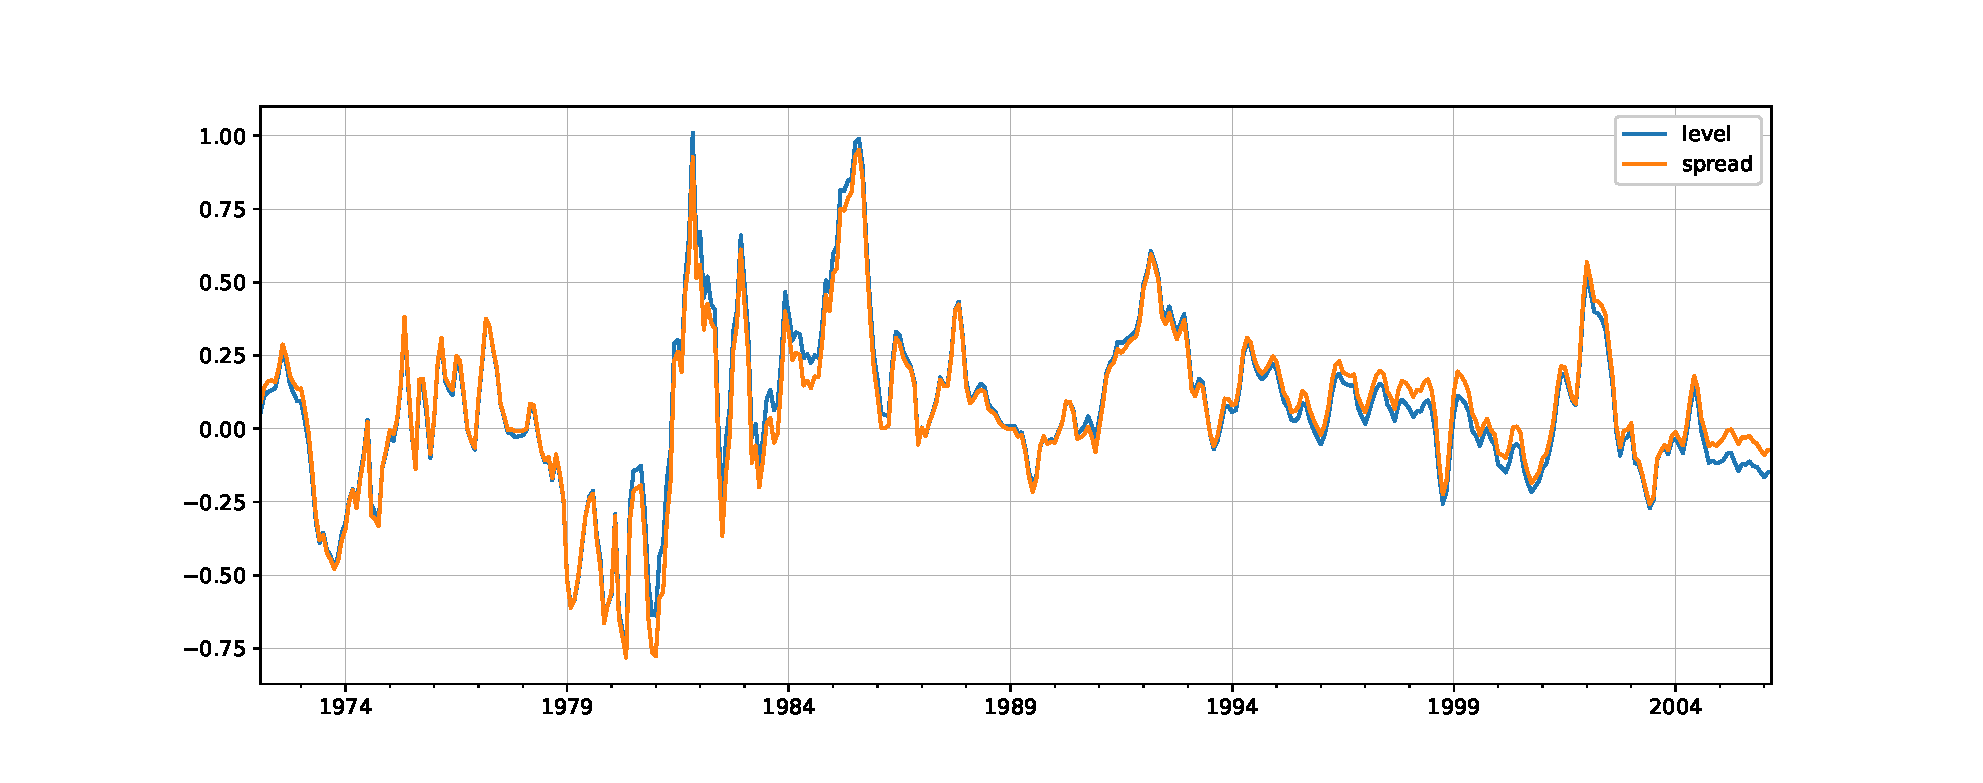
\includegraphics[scale=0.5]{fig/eps/Figure4.eps}
\end{figure}

\subsection{The Return-Forecast Factor is not Subsumed in Level, Slope and Curvature}

Another question that should be asked here is how well we can forecast excess returns using conventional yield curve factors. To do so, I replicate Table \ref{tab:2}, in which there's a comparison between the forecasting performance of the return-forecast factor with that of the conventional yield curve factors. To cosntruct these factors, they perform an eigenvalue decomposition of the covariance matrix of forward rates, $Q\Lambda Q^\T = \text{cov}(f_t)$ and then form factors using the formulae
\begin{equation}
	z_{it} = Q\left(:,i\right) f_t
\end{equation}
The main difference between my results and theirs is that I already get a high $\R^2$ when using the three factors \emph{level, slope} and \emph{curvature} (around 0.46), whilst they only get an $R^2$ of 0.34 when using the 5 factors. This difference should be studied a bit more.

\subsection{Fitting forwards - Risk Neutral Dynamics}
\begin{table}[h!]
	\centering
	\caption{Regression coefficients, $t$-statistics, $p$-values and $R^2$ for forecasting the average (across maturity) excess return $\bar{rx}_{t+2}$ in GSW data, based on the return-forecast factor $x_t$ and eigenvalue-decomposition factors of forward rates.}\label{tab:2}
	\input{tab/table2.txt}
\end{table}

Now I replicate the Figure \ref{fig:5}. Note that my results here are very poor (and so they are those by Cochrane and Piazzesi if they do what I am doing here, which can found in Cochrane's website), because I'm not computing the parameters and coefficients of the affine model using the minimisation but just the benchmark regression. Every single detail can be found in the code that I provide in my GitHub.
\begin{figure}[h!]
	\centering
	\caption{Affine model loadings $B^f$ in $f^{(n)} = A^f + \left(B^f\right)^\T X_t$. The line gives the loadings of the affine model, found by searching over parameters $\delta_0$, $\delta_1$, $\mu^\ast$ and $\phi^\ast$. }\label{fig:5}
	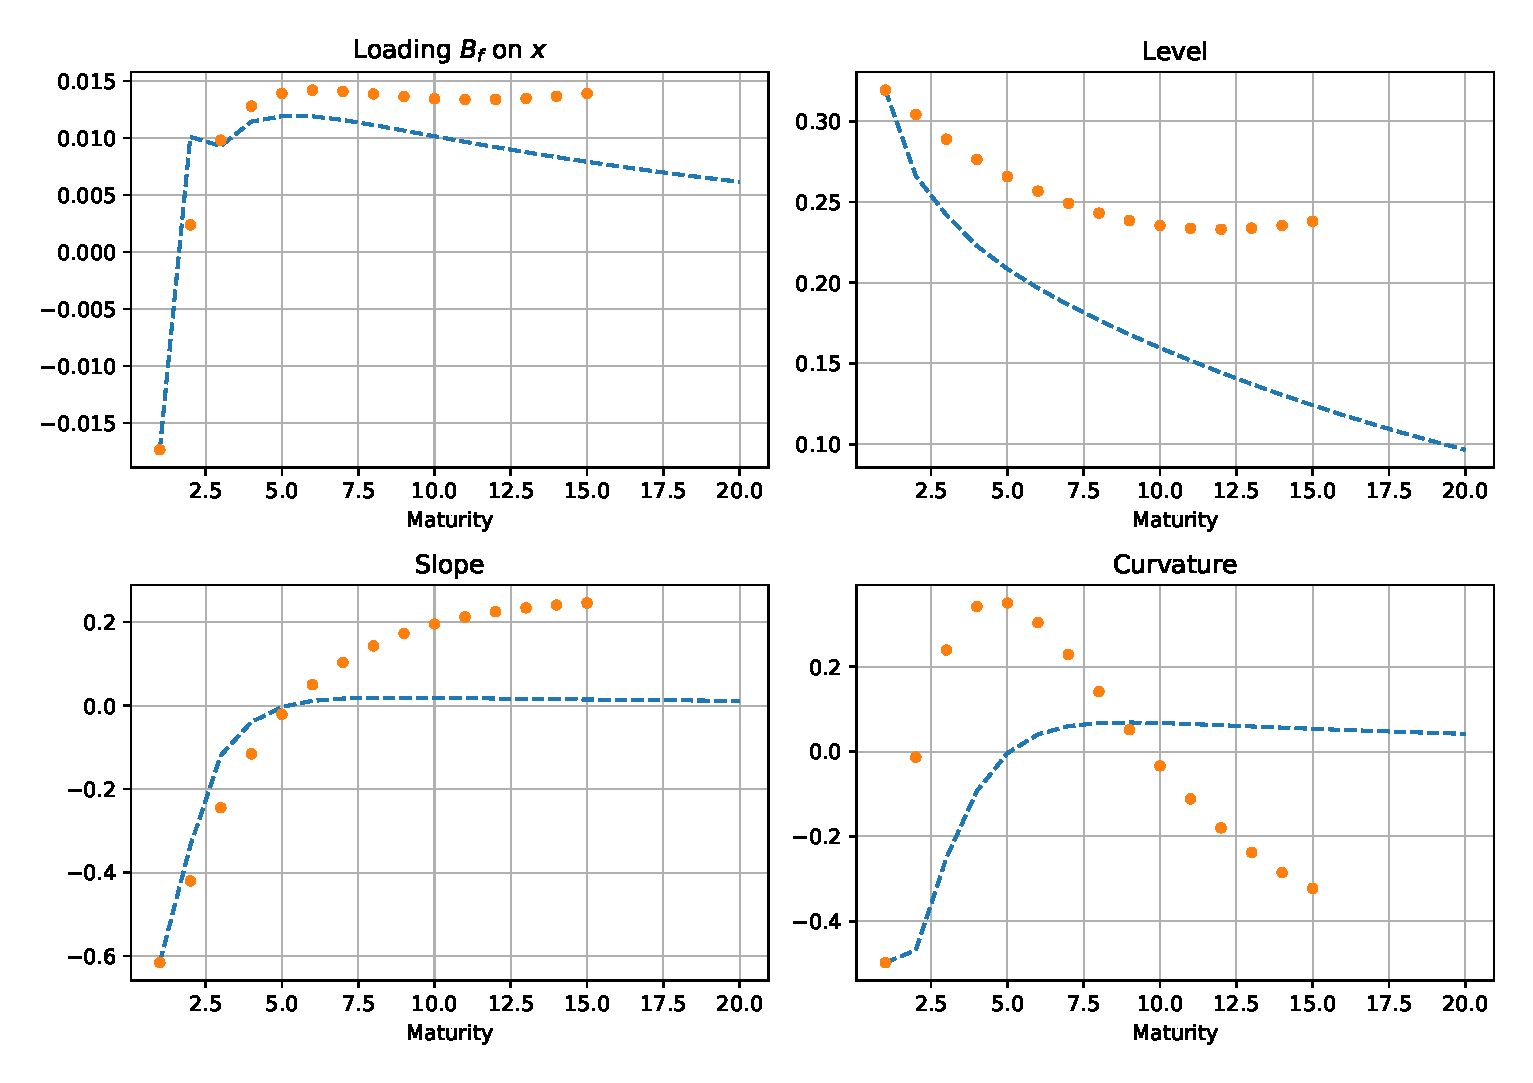
\includegraphics[scale=0.5]{fig/eps/Figure5.eps}
\end{figure}

\subsection{Market Prices of Risk}

Now I follow the procedure they describe to find the market prices of risk. What they do is to choose the market price of risk $\lambda_0$, $\lambda_1$ to match the cross-rection of bond expected returns. From the No Arbitrage restriction an the affine structure of the stochastic discount factor, we arrive to
\begin{equation}
	\E_t\left[rx_{t+1}\right] = \frac{1}{2}\sigma^2\left(rx_{t+1}\right) = \text{cov}\left(rx_{t+1}, v_{t+1}^\T\right) \left(\lambda_0 + \lambda_1 X_t\right).
\end{equation}
One of the main assumptions of this paper is that the model is conditionally homoskedastic, so $\sigma_t$ and $\text{cov}_t$ need nto $t$ subsprict. Hence, $\lambda_t$ gives the market price of risk of the $v_{t+1}$ shocks, i.e., it says how much an expected return must rise to compensate for covariance of that return with a given shock. Now remember (\ref{eq:28}). With this in our hands,
\begin{align}
		\left(I-q_rq_r^\T\right)\alpha + \frac{1}{2}\sigma^2\left(rx_{t+1}\right) &= \text{cov}_t\left(rx_{t+1}, v_{t+1}^\T\right) \lambda_0\\
		q_r &= \text{cov}\left(rx_{t+1}, v_{t+1}^\T\right)\lambda_{1x}
\end{align}
To understand the market prices of risk, they use the time-series of excess reutrns to estimate the variance term and that along with the time-series of factor shocks $v_{t+1}$ to estimate the covariance $\text{cov}_t\left(rx_{t+1}, v_{t+1}^\T\right)$. In Figure~\ref{fig:6}, I perform a cross-sectional regression to find the linear combination of the four covariance lines that most closely matches the expected return line. The graph shows that the expected return line is almost a perfect match to the covariances with the level shock. The others have completely a wrong shape. Hence, they set the market prices of risk other than level shock to zero.
\begin{figure}[h!]
	\centering
	\caption{Loading $q_r$ of expected returns on the return-forecasting factor $x_t$, covariance of returns with factor shocks, and fitted values. The fitted value is the OLS cross-sectional regression of $q_r$ on $\text{cov}\left(r, v_{level}\right)$, the dashed line nearly colinear with $q_r$. The covariance lines are rescaled to fit on the graph.}\label{fig:6}
	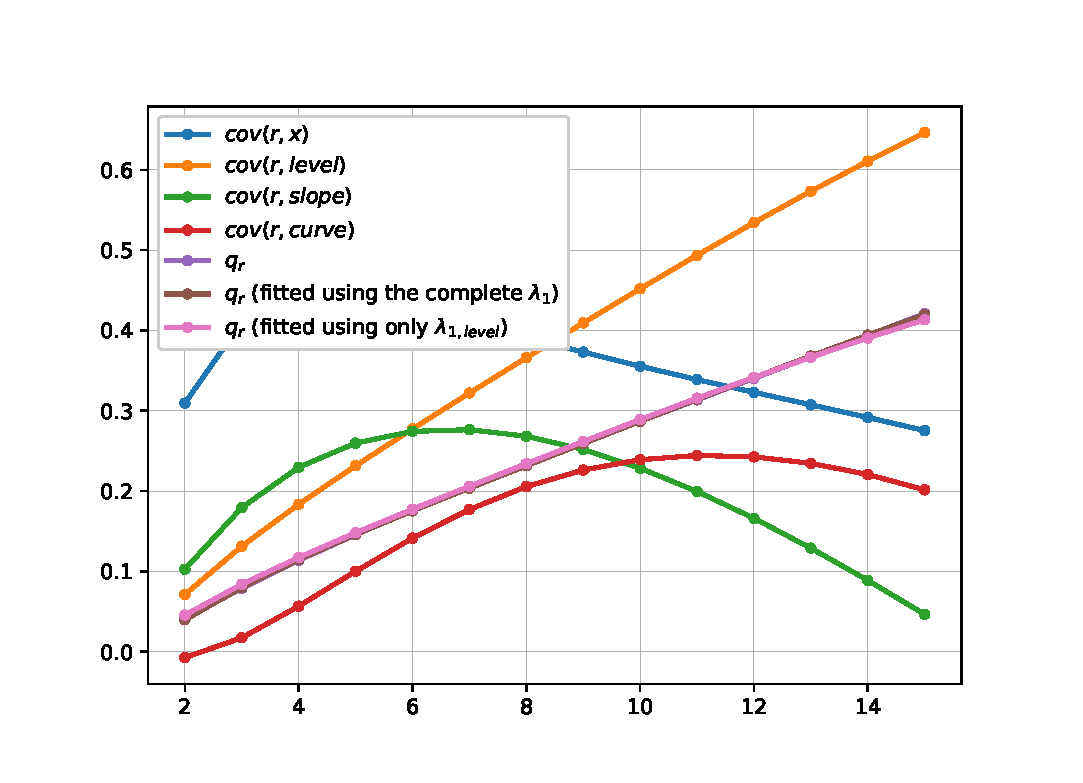
\includegraphics[scale=0.5]{fig/eps/Figure6.eps}
\end{figure}

\subsection{Transition matrices $\mu,\phi$, and impulse-response functions}

\begin{table}[h!]
	\centering
	\caption{Correlation matrix of shocks $V$, in $X_{t+1} = \mu + \phi X_t + v_{t+1}$, with $V = \text{cov}\left(v_{t+1}v_{t+1}^\T\right)$. OLS estimates.}\label{tab:5}
	\input{tab/table5.txt}
\end{table}


In this section I present the estimates of the transition matrices $\mu$ and $\phi$. The details of the equations can be found in the paper. In Table \ref{tab:4}, I present the risk-neutral dynamics, $\phi^\ast$. One thing that should be noted is that $\phi$ and $\phi^\ast$ only difffer in their first column, and in a constrained way, according to the covariance of shocks with the level shock. Note as well that the bottom two elements are nearly zero (shocks other than $x$ and level are nearly uncorrelated), so they only differ in the first two elements, actually. This is probably one of the most important points of the paper, since the transition dynamics built on time-series evidence are subject to substantial stastical uncertainty. Estimates of the risk-neutral dynamics are, by contrast, measured with high precision.
\begin{table}[h!]
	\centering
	\caption{Estimates of model dynamics, $\mu$ and $\psi$ in $X_{t+1} = \mu + \phi X_t + v_{t+1}$.}\label{tab:4}
	\input{tab/table4.txt}
\end{table}

In Figures \ref{fig:7} and \ref{fig:8}, I provide the responses $X_{t+1} = \phi X_t$ that follow from each element of $X$ being set to one with the others zero in turn. They do not orthogonalise the shocks, although only level and return forecast shocks have much correlation (Table \ref{tab:5}). All the descriptions of the impulse response functions can be found in the paper. I replicate them almost perfectly. The biggest difference is in the slope shock in Figure \ref{fig:7}. Note also that results have been scaled to fit in the graph, and I probably not choose the same scaling factors.



\begin{figure}[h!]
	\centering
	\caption{Impulse-response function of risk-neutral transition matrix $\phi^\ast$. The $x$ response is divided by two to fit on the same scale.}\label{fig:7}
	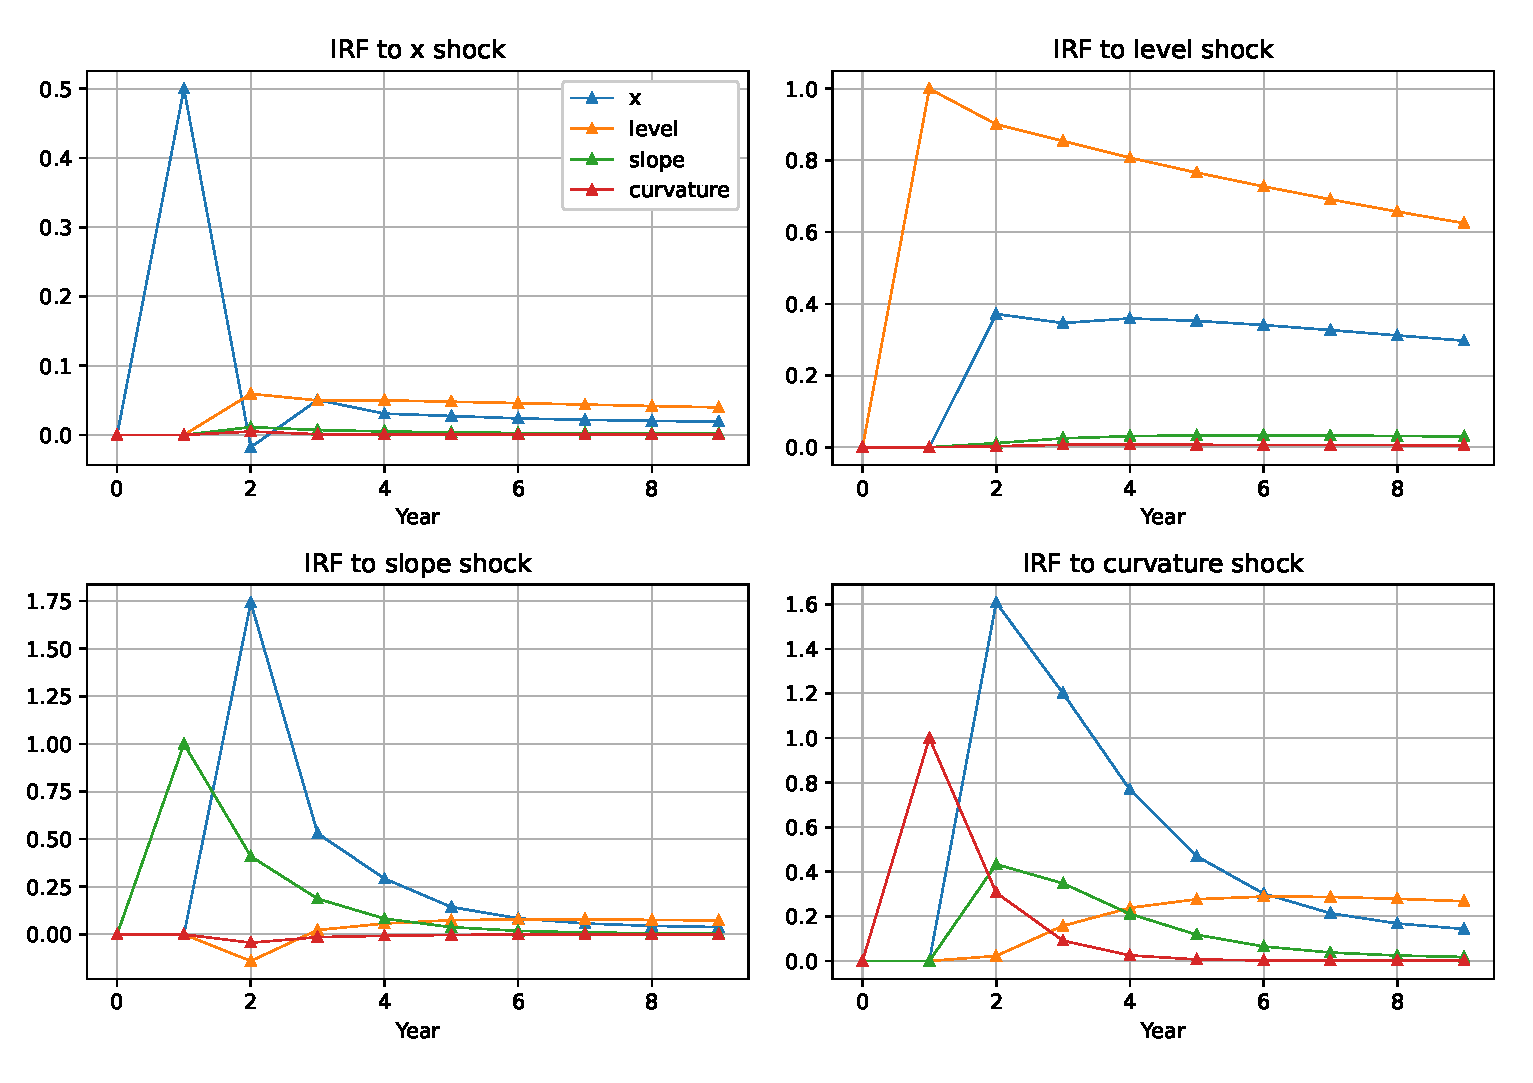
\includegraphics[scale=0.5]{fig/eps/Figure7.eps}
\end{figure}

\begin{figure}[h!]
	\centering
	\caption{Impulse-response function of real-measure transition matrix $\phi^\ast$. The $x$ response is divided by two to fit on the same scale.} \label{fig:8}
	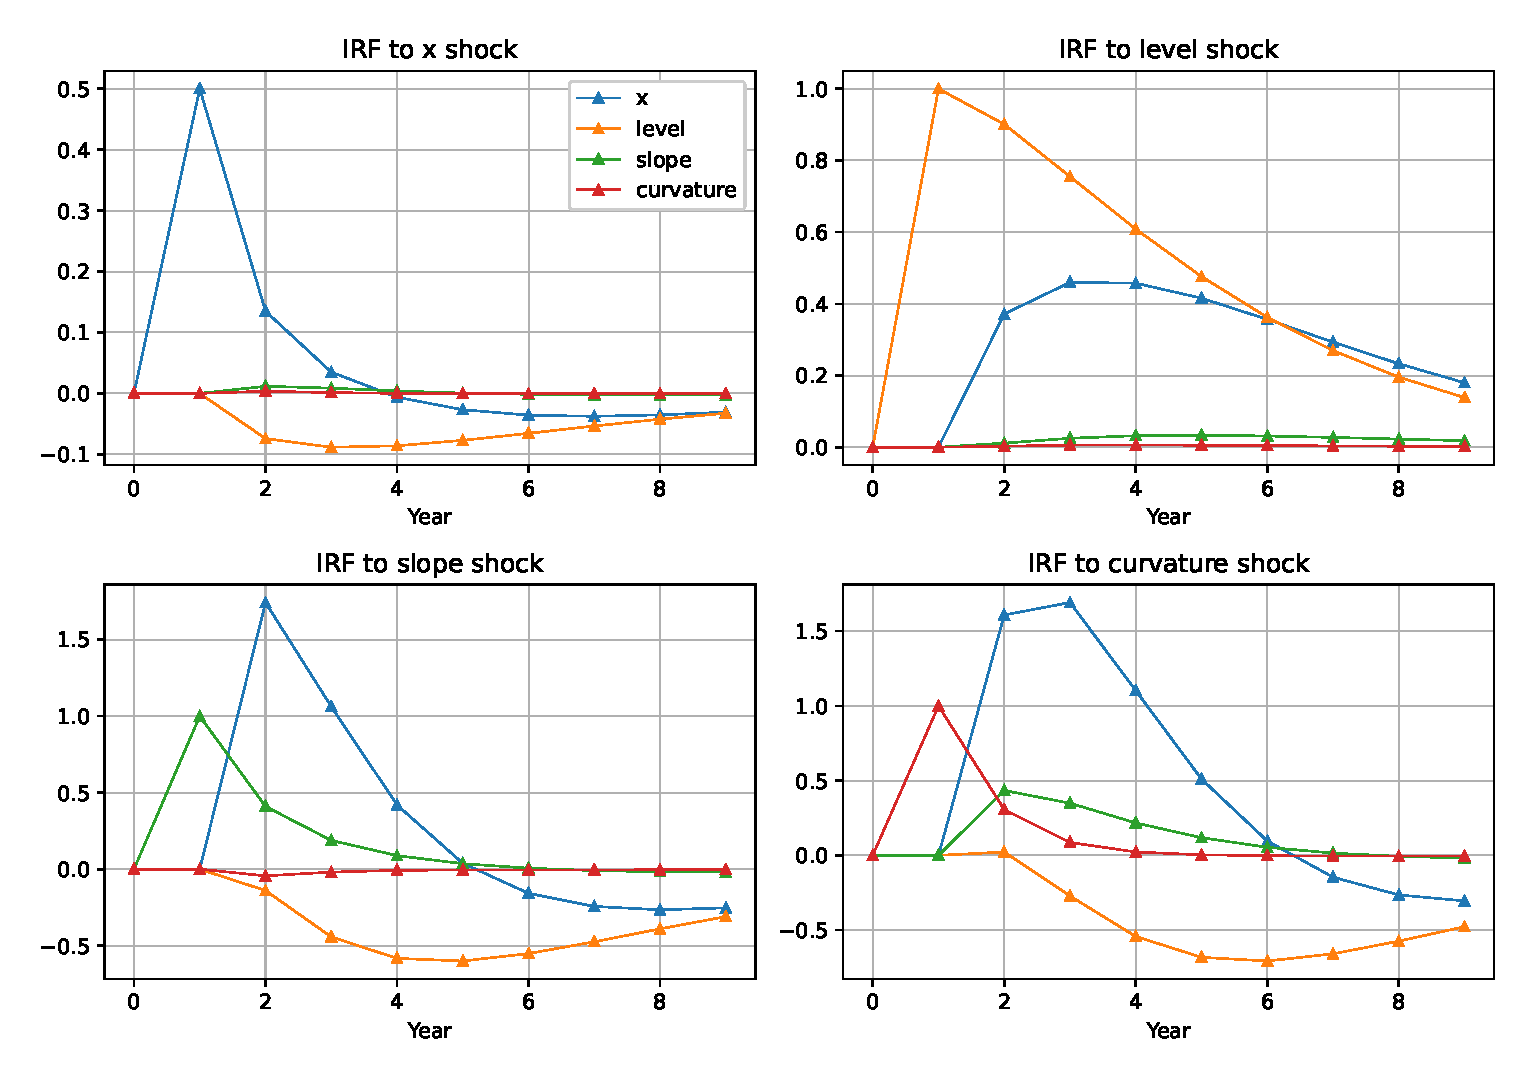
\includegraphics[scale=0.5]{fig/eps/Figure8.eps}
\end{figure}

Finally, I also provide Figures \ref{fig:9} and \ref{fig:10}, which plot responses of expected one year yields $\E_t\left[y_{t+n-1}^{(1)}\right]$, current forward rates $f_t^{(n)}$ and the expected future return-forecast factor $x_t$ to each fo the factor shocks. Note that under risk-neutral dynamics, the response of expected future yields is the same as the response of current forward rates up to a scaling factor. Also, a change in the return forecast factor quietly decays (top left panel of Figure \ref{fig:9}, and a change in the level factor sends current forward rates and expected future interest rates up for a long maturity and time. Slope and curvature shocks lead to sensibly shaped movements in expected future rates and current yields. In Figure \ref{fig:10}, we cans ee the crucial divergentce between current forward rates and expected future interest rates, which is a central question for a yield curve decomposition (not done). Here, we can see that the forward curve decomposition  at any date depends on factor congigurations at each date. Also, if there's a large return-forecast factor $x_t$ and the other factors are zero, current forwards are nearly constant. More comments can be found in the paper. The rest of the paper (decomposition and variations) is not covered in this replication.
\begin{figure}[h!]
	\centering
	\caption{Response of expected future one-year yield, current forward rates, and return-forecast factor $x$ to unit shocks, under the risk-neutral transition matrix.}\label{fig:9}
	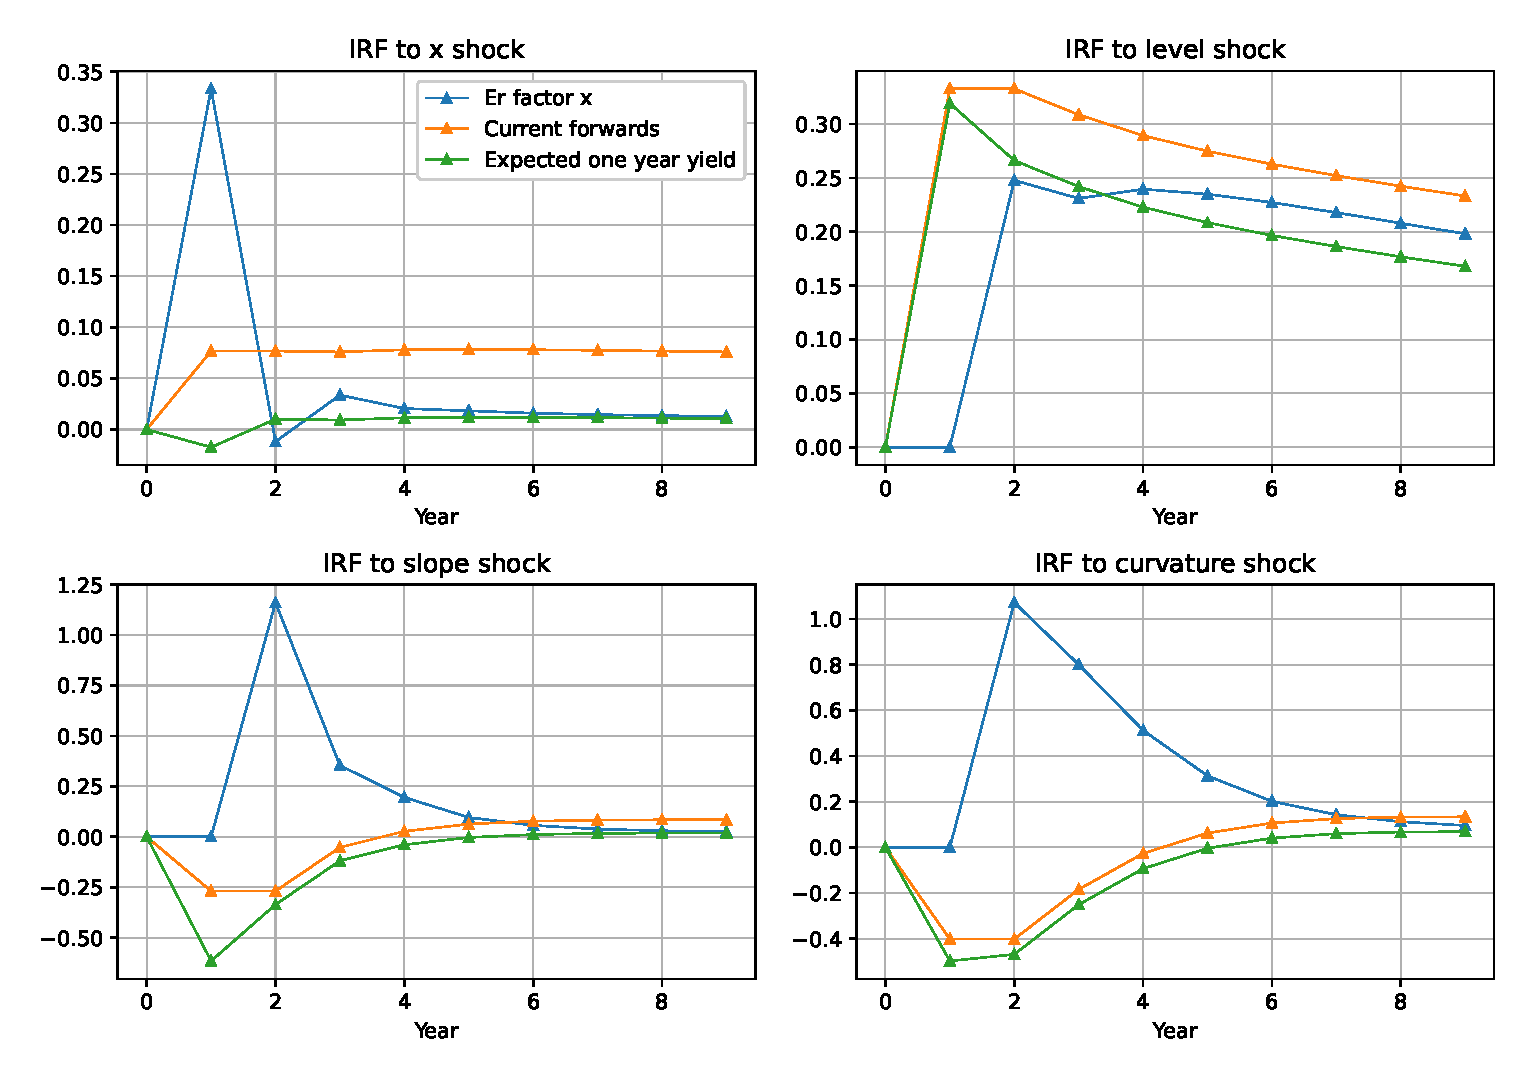
\includegraphics[scale=0.5]{fig/eps/Figure9.eps}
\end{figure}


\begin{figure}[h!]
	\centering
	\caption{Response of expected future one-year yield, current forward rates, and return forecast factor $x$ to unit shocks, under the estimated transition matrix $\phi$.}\label{fig:10}
	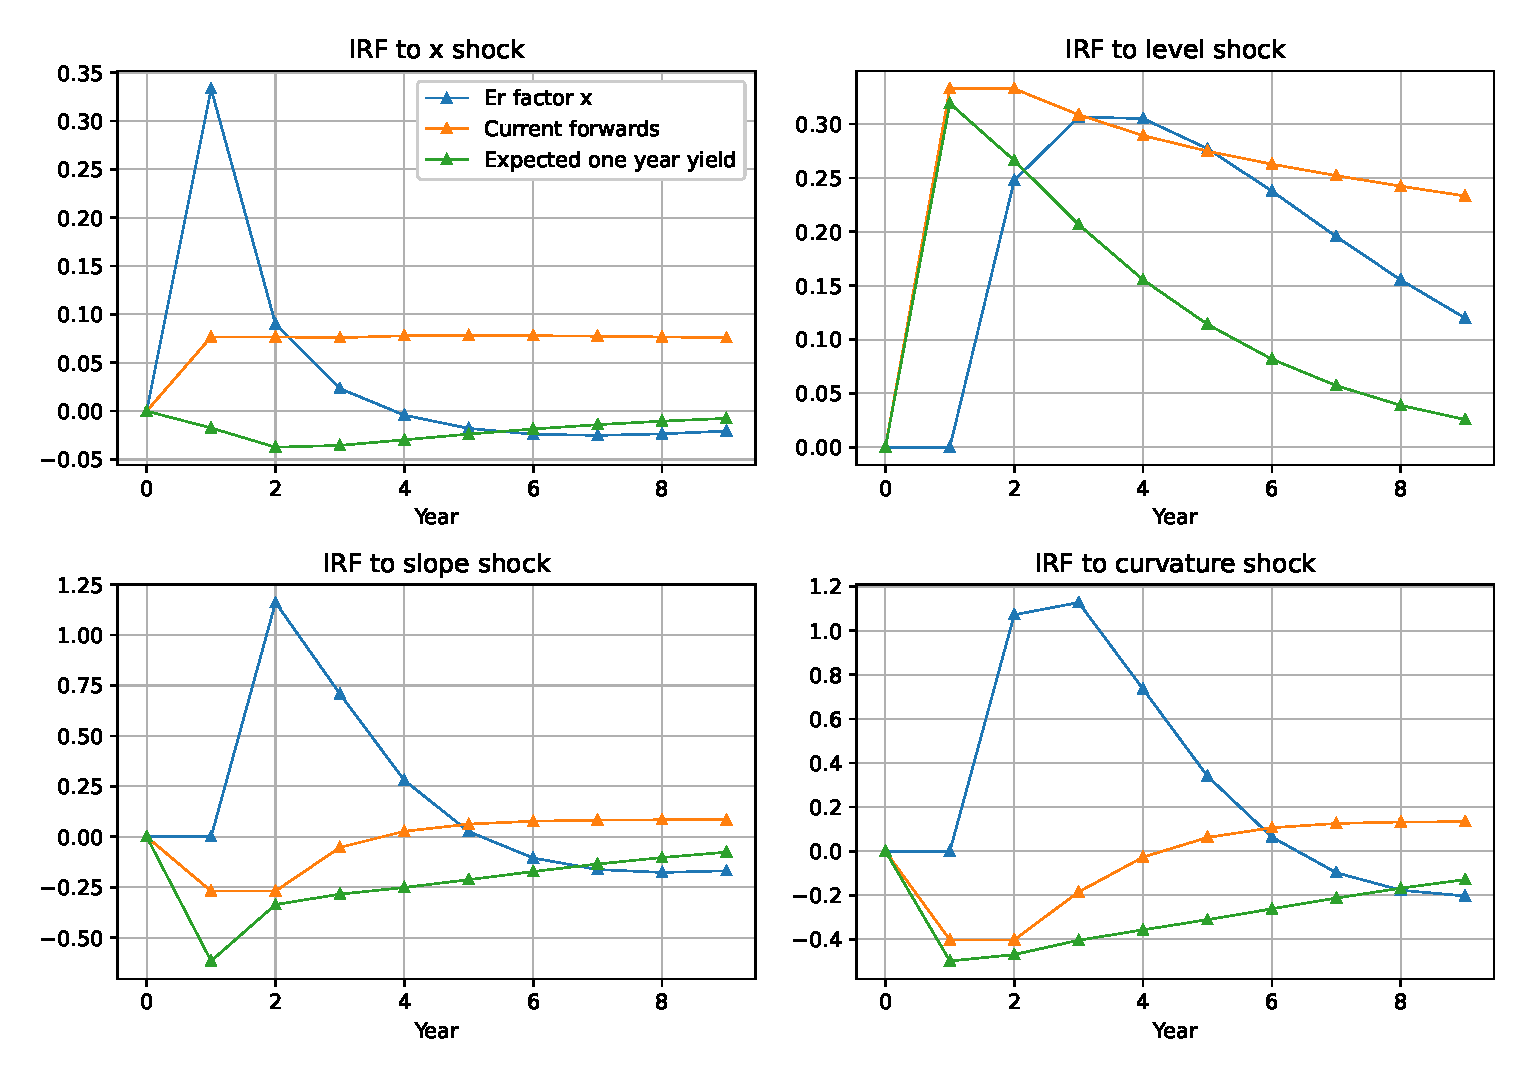
\includegraphics[scale=0.5]{fig/eps/Figure10.eps}
\end{figure}
